% !TeX spellcheck = en_GB

\section{Extending the Neural Engineering Framework}
\label{sec:nef_extension}

Up to this point, we have formally defined dendritic computation and discussed its theoretical benefits.
The goal of this section is to open avenues toward systematically integrating multi-compartment neuron models with dendritic trees into \NEF networks using the formalisms discussed above.

Na\"ively, incorporating neurons with multiple nonlinear input channels into the \NEF is merely a matter of solving for $\vec w$ such that \Cref{eqn:dendritic} holds.
Phrasing this as an optimisation problem, we must minimise the difference between the desired average activity according to the normative tuning-curve constraint $a_i(\vec x)$, and the average activity according to our multi\-variate response curve $\mathscr{G}$.
Using a least-squares loss (and omitting the regularisation term), we have
\begin{align}
	\begin{aligned}
	E &=
	\frac{1}{\vol(\Xrepr)} \int_{\Xrepr} \Bigl( a_i\bigl(\phi(x_1, \ldots, x_\ell)\bigr) -
	\mathscr{G} \bigl[
		\langle \vec w_{1, i}^1, \vec a^\mathrm{pre}_1(x_1) \rangle + \ldots +
		\langle \vec w_{\ell, i}^1, \vec a^\mathrm{pre}_\ell(x_\ell) \rangle, \ldots,\\
	&~\hspace{13.825em}
		\langle \vec w_{1, i}^k, \vec a^\mathrm{pre}_1(x_1) \rangle + \ldots +
		\langle \vec w_{\ell, i}^k, \vec a^\mathrm{pre}_\ell(x_\ell) \rangle
	\bigr] \Bigr)^2 \, \D x_1 \ldots \D x_\ell \,.
	\end{aligned}
	\label{eqn:dendritic_computation_optimisation}
\end{align}
One way to minimise this loss-function would be to use stochastic gradient descent.
In fact, this can be a viable strategy---and may be the only option for many detailed neuron models.

Still, we would like to suggest a more systematic approach that, in some cases, reduces the task of finding weights to a convex \qprog.
This is more in line with the \enquote{standard} \NEF, where connection weights are computed by solving a convex least-squares problem.

To arrive at a point where we can integrate complex neuron models more seamlessly, we first need to address two of the limitations of the \NEF discussed in \Cref{sec:nef_limitations}.
Specifically, we discuss how to eliminate the bias currents and to account for Dale's principle.
Furthermore, we present a modified version of \Cref{eqn:dendritic_computation_optimisation} that splits the multivarite response curve $\mathscr{G}$ into a multivariate input-dependent nonlinearity $H$ and a univariate response curve $G$.
We avoid decoding subthreshold currents using a technique we call \enquote{subthreshold relaxation}.

\subsection{Decoding the Current-Translation Function}
\label{sec:nef_decode_current}

So far we assumed that the current translation function $J_i(\xi)$ is an intrinsic part of the neuron model.
Our typical choice of $J_i(\xi) = \alpha_i \xi + \beta_i$ introduces a bias current $\beta_i$ into each neuron.
As we elaborated in \Cref{sec:nef_limitations}, this is slightly implausible from a biological perspective.

\Citet{tripp2007neural} demonstrate that it is possible to robustly solve for synaptic weights that approximate arbitrary post-synaptic current functions.
We use this insight to directly approximate the target current $J_i(\langle \vec e_i, \vec x \rangle)$; as a side effect, we implicitly solve for the bias.
Again, assuming that the post-synaptic current is linear in the pre-population activities, we must find a weight vector $\vec w_i$ such that the following regularised loss is minimised
\begin{align}
E = \frac{1}{\vol(\Xrepr)} \int_{\Xrepr} \left( J_i\bigl(\langle \vec e_i, \phi(\vec x)\rangle\bigr) - \langle \vec w_i, \vec a^\mathrm{pre}(\vec x) \rangle \right)^2 \, d\vec x + \lambda \| \vec w_i \|_\mathrm{2}^2\,.
\label{eqn:decode_current}
\end{align}
As before, this equation can be discretised, brought into canonical least squares form, and solved using the regularised Moore-Penrose pseudo inverse (cf.~eqn.~2.22 and 2.23):
\begin{align*}
	\mat W &= \mat A^+ \mat J \,, & \text{where} \quad \mat A^+ &= (\mat A^T \mat A + \lambda N \mat I)^{-1} \mat A^T \,.
\end{align*}
Here, $N$ is the number of samples, $\mat W \in \mathbb{R}^{m \times \Npop}$ is the connection weight matrix, $\mat J \in \mathbb{R}^{N \times m}$ is a matrix of target currents, and $\mat A \in \mathbb{R}^{N \times n}$ is the matrix of pre-activities.

\begin{figure}
	\includegraphics{media/chapters/03_nlif/03_02/current_translation_decoding.pdf}%
	{\phantomsubcaption\label{fig:current_translation_decoding_a}}%
	{\phantomsubcaption\label{fig:current_translation_decoding_b}}%
	{\phantomsubcaption\label{fig:current_translation_decoding_c}}%
	{\phantomsubcaption\label{fig:current_translation_decoding_d}}%
	\caption[Decoding for currents instead of represented values]{Decoding for currents instead of represented values. \textbf{(A)} Tuning curves of a pre-population with $100$ \LIF neurons (only $50$ tuning curves are shown). \textbf{(B)} Decoding affine current translation functions $J_i$ (dotted lines are the target). The function $\phi$ being computed in re\-pre\-sen\-tat\-ion space is the identity function. Dashed line corresponds to the threshold current $J_\mathrm{th} = \SI{1}{\nano\ampere}$.
	\textbf{(C)} Same as \emph{(B)} but for Gaussian current-translation functions $J_i$. Such functions can be used to produce localised tuning curves.
	\textbf{(D)} First six singular values of the two weight matrices $\mat W$ from \emph{(B, C)}.
	Singular values are normalised by dividing by their sum, resulting in the relative contribution of each singular value to the decoding.
	For affine $J_i$, $\mat W$ is of rank $d + 1$ (here $d = 1$);
	Gaussian $J_i$ result in full-rank $\mat W$.
	}
\end{figure}

Importantly, we no longer solve for weights directly in the domain of represented values $\vec x$; this is in contrast to solving for decoders $\mat D$ according to \cref{eqn:lstsq_loss}.
Similarly, we do not solve for target activities $a_i$, as was suggested by our na\"ive loss function in \cref{eqn:dendritic_computation_optimisation}.
Side-stepping the neural nonlinearity $G$ enables a simple least-squares solution.
Furthermore, this optimisation scheme supports arbitrary current-translation functions $J_i$, providing modellers with a greater flexibility over the tuning curve constraint (cf.~\Cref{fig:current_translation_decoding_a,fig:current_translation_decoding_b,fig:current_translation_decoding_c}).

\subsubsection{Low-rank factorisation of $\mat W$}
Solving the optimisation problem in \cref{eqn:decode_current} directly results in a weight matrix $\mat W$ instead the low-rank factorisation $\mat W = \mat E \mat D^\phi$.
As discussed in \Cref{sec:nef_transformation}, this factorisation was useful, since it enables $\mat W \vec a$ to be computed in $\mathcal{O}(n)$ instead of $\mathcal{O}(n^2)$.

Fortunately, at least in the case of the affine current-translation function $\alpha_i \langle \vec e_i, \phi(\vec x) \rangle + \beta_i$, we still obtain a factorisable matrix (cf.~\Cref{fig:current_translation_decoding_d}).
The resulting $\mat W$ is merely of rank $d + 1$, where $d$ is the dimensionality of the post-population.
Specifically, the weight matrix can be expressed as a sum of the low-rank factorisation $\mat E \mat D^\phi$ and the outer product of the biases $\vec \beta \in \mathbb{R}^{m \times 1}$ with a decoding vector $\mat D^1 \in \mathbb{R}^{1 \times n}$.
This \enquote{bias-decoder} decodes the constant \enquote{one} from the pre-population.
In other words, it simply holds $\mat W = \mat E \mat D^\phi + \vec \beta \mat D^1$ (cf.~\cite[Chapter~4]{stockel2017point,duggins2017incorporating}).

\begin{figure}
	\includegraphics{media/chapters/03_nlif/03_02/bias_decoding_impact.pdf}%
	{\phantomsubcaption\label{fig:bias_decoding_impact_a}}%
	{\phantomsubcaption\label{fig:bias_decoding_impact_b}}%
	{\phantomsubcaption\label{fig:bias_decoding_impact_c}}%
	{\phantomsubcaption\label{fig:bias_decoding_impact_d}}%
	\caption[Bias decoding and post-population tuning curve accuracy]{Bias decoding and post-population tuning curve accuracy. \textbf{(A)} Pre-population tuning-curves for $n = 50$ \LIF neurons.
	\textbf{(B)}~Error for decoding the identity function compared to decoding a constant (regularisation factor $\sigma = 10$). The error for decoding a constant is minimally larger than that for decoding the identity function.
	\textbf{(C)}~The first four principal components of the tuning curves (for $n = 1000$).
	The principal components resemble the Legendre polynomials, an orthogonal function basis (dotted lines).
	\textbf{(D)} \RMSE between the desired post-population tuning and the actually achieved tuning. Decoding the bias approximately doubles the error compared to intrinsic bias currents.}
\end{figure}

\subsubsection{Impact of decoding bias currents on network function}
%It is difficult to make blanket statements about the impact of bias decoding on the network function.
Generally speaking, decoding biases increases the error between the actual and desired post-population tuning.
The magnitude of this error depends on the pre- and post-population. 
The former determine how well a constant offset can be decoded, the latter determine the magnitude of the required bias currents.

In the case of \enquote{standard} \NEF tuning with uniform $x$-intercepts and random encoders (cf.~\Cref{fig:bias_decoding_impact_a}), constant functions can, counter-intuitively, only be decoded with a slightly higher error than the identity function (error is about $15\%$ higher; cf.~\Cref{fig:bias_decoding_impact_b}).
This becomes apparent when considering the principal components of the pre-population tuning curves.
As, for example, discussed in \citet[Chapter~7]{eliasmith2003neural}, the principal component analysis (PCA) can be seen as \enquote{uncovering} the best orthogonal basis that linearly generates the tuning-curves.
%(see \cite[Chapter~12]{bishop2006pattern} for general information on the PCA).
In turn, the first principal components characterise the functions that can be decoded well from a population.
As illustrated in \Cref{fig:bias_decoding_impact_c}, the principal components $f_i$ of the \enquote{standard} \NEF tuning curves resemble the Legendre polynomials (cf.~\Cref{sec:function_bases} for a definition).
While the second principal component $f_2$ is linear, just like the corresponding Legendre polynomial, $f_1$ differs significantly from the constant first Legendre polynomial.
Decoding constants is hence \enquote{more difficult} than decoding the identity function.

In our example, and as depicted in \Cref{fig:bias_decoding_impact_d}, decoding $J_i$ doubles the \RMSE between the desired and actual post-population tuning.
%This can be countered by doubling the number of pre-neurons.
However, as we will see in the next subsection, there are circumstances where the absence of an intrinsic bias improves the network performance.

\subsubsection{Accounting for multiple pre-populations}
As we discussed in \Cref{sec:additive_net}, a welcome side effect of intrinsic current-translation is that standard \NEF networks are additive.
Summing the activities $\vec a^\mathrm{pre}_1$, $\ldots$, $\vec a^\mathrm{pre}_\ell$ from multiple pre-populations is equivalent to summing the decoded $f_1(\vec x_1)$, $\ldots$, $f_\ell(\vec x_\ell)$.
This is no longer the case when
%solving for weights $\vec w_i$
minimising the current-based loss in \cref{eqn:decode_current}.

\begin{figure}
	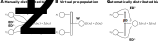
\includegraphics{media/chapters/03_nlif/03_02/nef_decode_bias.pdf}%
	{\phantomsubcaption\label{fig:nef_decode_bias_a}}%
	{\phantomsubcaption\label{fig:nef_decode_bias_b}}%
	{\phantomsubcaption\label{fig:nef_decode_bias_c}}%
	\caption[Accounting for multiple pre-populations when decoding the current-translation function]{Accounting for multiple pre-populations when decoding the current-translation function. \textbf{(A)} Biases can be manually distributed between pre-populations by scaling the bias decoders $\mat D^1_1$ and $\mat D^1_2$ by $\alpha$ and $(1 - \alpha)$, respectively. \textbf{(B)} The general solution is to solve for weights $\mat W$ assuming stacked pre-population activities. The two pre-populations form a \enquote{virtual} pre-population. \textbf{(C)} A combination of the two approaches, where only the bias $\mat D^1$ is decoded from the pre-populations in this way.}
\end{figure}

In the case of the affine $J_i$, each of the $\ell$ connections decodes the bias current, effectively multiplying the bias by $\ell$.
Of course, we can only decode a fraction of the bias from each pre-population (\Cref{fig:nef_decode_bias_a}).
Alternatively, we can combine the pre-populations into a \enquote{virtual pre-population} and let the optimisation process take care of distributing the responsibility for providing the bias between all pre-neurons (\Cref{fig:nef_decode_bias_b}).

More precisely, we explicitly solve for weights that result in $f_1(\vec x_1) + \ldots + f_\ell(\vec x_\ell)$ to be represented in the post-population.
For two populations, and skipping regularisation, we have
\begin{align}
	E =
	\frac{1}{\vol(\Xrepr)^2} \! \iint_{\Xrepr}
	\left(
		J_i\bigl(\langle \vec e_i, f_1(\vec x_1) + f_2(\vec x_2) \rangle\bigr)
		- \langle \vec w_{1, i}, \vec a_1^\mathrm{pre}(\vec x_1) \rangle
		- \langle \vec w_{i, 2}, \vec a_2^\mathrm{pre}(\vec x_2) \rangle
	\right)^2 \, \D\vec x_1 \D\vec x_2 \,.
	\label{eqn:decode_current_additive}
\end{align}
We can bring this problem into a canonical form by stacking the pre-activities and weights (see below for an example).
However, note that we now need to sample a much higher-dimensional space.
This is worrisome if we attempt to decode $f_i$ that must be finely sampled to obtain a good decoding.
Again, under the assumption that $J_i$ is affine, it is possible to expand the above integral and to solve for a---relatively easy to decode---population-spanning bias decoder $\mat D^1$ independent of the (untouched) function decoders $\mat D^{f_1}$ and $\mat D^{f_2}$ (\Cref{fig:nef_decode_bias_c}).

%\begin{align*}
%E^\beta &= \frac{1}{\vol(\Xrepr)^2} \! \int_{\Xrepr} \! \int_{\Xrepr} \left( \beta_i - \langle \vec w^\beta_{1, i}, \vec a_1^\mathrm{pre}(\vec x_1) \rangle - \langle \vec w^\beta_{i, 2}, \vec a_2^\mathrm{pre}(\vec x_2) \rangle \right)^2 \, d\vec x_1 \, d\vec x_2
%\end{align*}

\subsection{Nonnegative Weights and Dale's Principle}
\label{sec:nef_nonneg}

Biological neurons tend to follow Dale's principle---they act either excitatorily or inhibitorily (see~\Cref{sec:synaptic_transmission} for more detail).
As discussed in \Cref{sec:nef_limitations}, we ignored this in our weight-solving procedures.
Least-squares assigns arbitrary algebraic signs to the individual weights, typically with an even split between positive and negative (cf.~\Cref{fig:sparsity_and_dales_principle}).
Such weights are not compatible with conductance-based synapses or, more generally, multi-compartment neurons, where modellers may connect pre-neurons to specific post-neuron channels.
The corresponding connection weights describe nonnegative quantities, such as the number of vesicles released from the pre-synapse, or the channel density in the post-synapse \citep{roth2009modeling}.

\subsubsection{Solving for weights using nonnegative least squares}
Solving for individual synaptic weights in current space suggests a simple procedure to account for nonnegativity.
Assume that each population is arbitrarily split into a group of excitatory and inhibitory neurons.
The somatic input current of post-neuron $i$ in response to pre-synaptic activity is $\langle \vec w_i^+, \vec a^+(\vec x) \rangle - \langle \vec w_i^-, \vec a^-(\vec x) \rangle$;
here, $\vec w_i^+$, $\vec w_i^-$ are nonnegative excitatory and inhibitory weight vectors and $\vec a^+(\vec x)$, $\vec a^-(\vec x)$ are the activities of the excitatory and inhibitory neurons in the pre-population.
Combining this current term with \cref{eqn:decode_current} yields the following optimisation problem for each post-neuron $i$
\begin{align}
	\begin{aligned}
	& \min_{{\vec w}_i^+, {\vec w}_i^-}
	\frac{1}{\vol(\Xrepr)} \int_{\Xrepr} \!
	\left(
		J_i\bigl(\langle \vec e_i, \phi(\vec x) \rangle\bigr)
		- \langle \vec w_{i}^+, \vec a^+(\vec x) \rangle
		+ \langle \vec w_{i}^-, \vec a^-(\vec x) \rangle
	\right)^2 \, \D \vec x + \sigma^2 \|\vec w_{i}^+\|_2^2 + \sigma^2 \|\vec w_{i}^-\|_2^2 \\
	& \text{subject to } \vec w_i^+, \vec w_i^- \geq 0 \,.
	\end{aligned}
	\label{eqn:decode_nonneg}
\end{align}
To obtain a canonical least-squares form, let $N$ be the number of samples, $n^+$, $n^-$ be the number of excitatory and inhibitory pre-neurons,%
\footnote{
It does not necessarily hold that $n = n^+ + n^-$; neurons can \emph{technically} be marked as both excitatory and inhibitory. Specifically, the special case $n = n^+ = n^-$ reduces the \NNLS problem to standard least squares.
}
and $\mat A$ be the sampled, stacked, and signed pre-activities $(\mat A^+, -\mat A^-) \in \mathbb{R}^{N \times (n^+ + n^-)}$.
Additionally, let $\mat W$ be the stacked weight matrices $(\mat W^+, \mat W^-) \in \mathbb{R}^{(n^+ + n^-) \times m}$, and $\vec J \in \mathbb{R}^{N \times m}$ be a matrix of sampled target currents. We have
\begin{align}
	\bigl\| \bigl( \mat A^T \mat A + N \sigma^2 \mat I \bigr) \mat W - \mat A^T \mat J \bigr\|_2^2 \quad\quad \text{subject to } \mat W \geq 0 \,.
	\label{eqn:decode_nonneg_canon}
\end{align}
This is a standard nonnegative least-squares (\NNLS) problem that can be solved in polynomial time \citep[Chapter~23]{lawson1995solving}.
An overview of efficient algorithms to solve this kind of problem is given in \citet{chen2009nonnegativity}.%
\footnote{Most linear algebra software packages bundle a solver for nonnegative least-squares; for example \texttt{scipy.optimize.nnls} in SciPy or \texttt{lsqnonneg} in Matlab. Alternatively, a general quadratic programming (\QP) solver can be used; this is what we do in our library \emph{libnlif} that we discuss in \Cref{app:libnlif}.}
Of course, similarly to \cref{eqn:decode_current_additive}, the optimisation problem can be extended to take multiple pre-populations into account.

\begin{figure}[p]
	\centering
	
\includegraphics{media/chapters/03_nlif/03_02/nonnegative_experiments_setup.pdf}\\[0.75cm]	\includegraphics{media/chapters/03_nlif/03_02/nonnegative_experiments.pdf}\\[0.75cm]
	\includegraphics{media/chapters/03_nlif/03_02/nonnegative_experiments_tuning.pdf}%
	{\phantomsubcaption\label{fig:nonnegative_experiments_a}}%
	{\phantomsubcaption\label{fig:nonnegative_experiments_b}}%
	{\phantomsubcaption\label{fig:nonnegative_experiments_c}}%
	{\phantomsubcaption\label{fig:nonnegative_experiments_d}}%
	{\phantomsubcaption\label{fig:nonnegative_experiments_e}}%
	\caption[Impact of the ratio between excitatory to inhibitory neurons on network function]{Impact of the ratio between excitatory to inhibitory neurons on network function.
	\textbf{(A)} A variable $x$ is represented in a pre-population. This population is randomly split into $n^+$ excitatory and $n^-$ inhibitory neurons. Nonnegative weights $\mat W^+$, $\mat W^-$ are optimised according to \cref{eqn:decode_nonneg_canon}. An identity decoder $\mat D$ is used to decode the value represented in the post-population.
	\textbf{(B, C)} Median normalised \RMSE (relative to the \RMS of $\phi(x)$) between the decoded value and the desired value $\phi(x) = x$ \emph{(B)} or $\phi(x) = 2x^2 - 1$ \emph{(C)} for different ratios $n^+ \!\! : \! n^-$ over $1000$ runs ($n = m = 100$, $\sigma = 10$, maximum rates between $50$ and $100$). The shaded area depicts the 25/75 percentiles. The dashed line depicts results for the intrinsic biases. The horizontal dotted line is the least-squares baseline.
	Except for extreme $n^+ \!\! : \! n^-$, the network works well over a large range of ratios.
	Intrinsic biases are detrimental in purely excitatory networks.
	\textbf{(D, E)} Examples of desired versus actual post-population tuning at different excitatory to inhibitory pre-neuron count ratios.
	A reasonably good post-population tuning can be obtained for purely excitatory pre-populations and a decoded (non-intrinsic) bias.
	}
	\label{fig:nonnegative_experiments}
\end{figure}

\subsubsection{Impact of nonnegative weights on network function}
The degree to which separating populations into excitatory and inhibitory sub-populations impacts network function once again depends on the pre- and post-population tuning, as well as the $\phi$ that we would like to compute.

We explore this in the network depicted in \Cref{fig:nonnegative_experiments}.
Decoding errors are small over a wide range of ratios between the excitatory and inhibitory pre-neurons.
However, without additional precautions (see below) information cannot be transmitted over purely inhibitory connections.
In contrast, purely excitatory connections can work reasonably well, at least when computing the identity function $\phi(x) = x$ and when decoding the bias from the pre-population.
We further reduce this error below, using \enquote{subthreshold relaxation}.

Note that purely excitatory connections do not work for the selected post-tuning in the presence of intrinsic bias currents.
The excitatory input cannot counter positive $\beta_i$ for neurons with negative $x$-intercepts, making it impossible to reach firing rates smaller than $a_i(\beta_i)$.%
\footnote{This phenomenon is also described in the documentation for the \texttt{Nnls} solver in Nengo. 
Our optimisation procedure differs from that in Nengo in that we account for excitatory and inhibitory pre-neurons and that we can choose to decode the current translation function, eliminating the post-population tuning restrictions.}

\subsubsection{Factorisability of nonnegative weight matrices}
As we discussed in the previous subsection, directly solving for weights $\mat W$ forfeits the computationally efficient low-rank factorisation $\mat W = \mat E \mat D^\phi$.
At least for affine $J_i$ it is possible to work around this using the bias decoder $\mat D^1$.

Such simple workarounds are no longer possible for nonnegative $\mat W^+$, $\mat W^-$.
Still, we can construct low-rank approximations of $\mat W^+$ and $\mat W^-$ using their singular value decomposition.
Generally, a rank-$k$ factorisation of a matrix $\mat M \in \mathbb{R}^{m \times n}$ can be obtained according to
\begin{align}
	\mat M_{(k)} = \sum_{i = 1}^k \sigma_k \vec u_k \vec v_k^T \,, \quad\quad
	\begin{aligned}	
		&\text{where } \mat U^T \mat \Sigma \mat V = \mat M \,
		\text{ and } \mat \Sigma = \mathrm{diag}(\sigma_1, \ldots, \sigma_{\min\{m, n\}}) \\
		&\text{with }
	\sigma_1 \geq \ldots \geq \sigma_{\min\{m, n\}}
	\end{aligned}
	\label{eqn:svd_factorisation}
\end{align}
According to the Perron-Frobenius theorem and generalisations thereof for square matrices \citep{avin2013generalized}, $\mat M_{(1)}$ is nonnegative if $\mat M$ is nonnegative (at least for practically relevant classes of $\mat M$).
Since $\sigma_1$ is the dominating singular value, and the $\sigma_k$ tend to decay quickly in magnitude, the higher-rank factorisations $\mat M_{(k)}$ will mostly be nonnegative. Still, nonnegativity of $\mat M_{(k)}$ is not guaranteed.
When factorising $\vec W^+$ and $\vec W^-$ in this manner, we hence suggest ensuring that the decoded currents $\vec J \in \mathbb{R}^{m}$ injected into the post-neurons are nonnegative, i.e.,
\begin{align*}
	\vec J = \max\bigl(0, \vec W^+_{(k)} \vec a^+ \bigr) - \max\bigl(0, \vec W^-_{(k)} \vec a^- \bigr) \,.
\end{align*}%
\begin{figure}
	\includegraphics{media/chapters/03_nlif/03_02/nonnegative_factorisation.pdf}
	\caption[Rank-reduced factorisation of nonnegative weight matrices]{Rank-reduced factorisation of nonnegative weight matrices. Same experiment as in \Cref{fig:nonnegative_experiments}, but for independently factorised and rank-reduced excitatory and inhibitory weight matrices $\mat W^+$, $\mat W^-$ (see text). Each curve corresponds to a sweep over the excitatory to inhibitory ratio (cf.~\cref{fig:nonnegative_experiments_b,fig:nonnegative_experiments_c}).
	\textbf{(A)} With intrinsic biases, the nonnegativity increases the effective rank of the weight matrices by one.
	\textbf{(B)} When decoding the biases, factorisations with higher ranks are required, particularly for purely excitatory connections (likely due to higher sparsity, see \cref{fig:nonnegative_sparsity_c}).}
	\label{fig:nonnegative_factorisation}
\end{figure}%
We explore this factorisation in \Cref{fig:nonnegative_factorisation}.
Typically, a relatively small $k \ll \min\{m, n\}$ suffices to obtain low decoding errors in the post-population.

\pagebreak

\subsubsection{Sparsity of nonnegative weight matrices}
The weight matrices returned by the nonnegative least-squares solver tend to be sparse.
This is, for example, quite apparent in our motivational illustration from the last chapter (\Cref{fig:sparsity_and_dales_principle}).
Interestingly, the sparsity of \NNLS solutions is not just an artefact of our particular problem domain.
\Citet{slawski2013nonnegative} show that, under certain circumstances, the nonnegativity constraint induces an implicit $L_1$ regularisation term $\lambda_1 \|\vec w_i\|_1$.
This kind of regularisation, also referred to as \enquote{lasso}, is a standard method for obtaining sparse solutions \citep[Section~3.1.4]{bishop2006pattern}.
If combined with our original $L_2$ regularisation term $\sigma^2 \| \vec w_i \|_2^2$, the resulting optimisation problem is also called \enquote{elastic net} \citep{zou2005regularization}.
The $L_2$ regularisation factor $\sigma^2$ accounts for Gaussian noise and ensures that the problem is non-singular, while the $L_1$ regularisation factor $\lambda_1$ encourages sparsity.

\begin{figure}
	\includegraphics{media/chapters/03_nlif/03_02/nonnegative_sparsity.pdf}%
	{\phantomsubcaption\label{fig:nonnegative_sparsity_a}}%
	{\phantomsubcaption\label{fig:nonnegative_sparsity_b}}%
	{\phantomsubcaption\label{fig:nonnegative_sparsity_c}}%
	\caption[Comparison of weight optimisation schemes in terms of sparsity]{Comparison of weight optimisation schemes in terms of sparsity.
	Curves (\emph{top}) depict sparsity and decoding errors over different hyperparameters (\emph{bottom}).
	Data are for decoding the bias current and $\phi(x) = x$ and are the median over $1000$ trials.
	Network, parameters, and error measure are the same as in \Cref{fig:nonnegative_experiments}.
	Weights with a magnitude below $10^{-6}$ are counted as zero.
	\textbf{(A)}~Solving for weights $\mat W$ according to \cref{eqn:decode_current} with enforced sparsity.
	Weights $\mat W$ with a magnitude below the $P$th percentile are set to zero; the weights are re-solved.
	Sparsity up to $25\%$ has no impact on the error; errors increase drastically for sparsities over $75\%$.
	\textbf{(B)}~Encouraging sparsity using an $L_1$ term (in addition to $L_2$ regularisation) results in lower errors compared to the enforced sparsity.
	\textbf{(C)}~Solving for nonnegative $\mat W^+$, $\mat W^-$ using \cref{eqn:decode_nonneg_canon}.
	For a large range of excitatory to inhibitory ratios this results in a sparsity of about $50\%$, with errors similar to $L_1$ regularisation for the same sparsity.
	}
	\label{fig:nonnegative_sparsity}
\end{figure}

Indeed, as we explore in \Cref{fig:nonnegative_sparsity}, the \NNLS solution has sparsity of about $50\%$.
Notably, this is the case over a wide range of excitatory to inhibitory ratios; sparsity is \emph{not} just a result of the solver requiring certain pre-neurons to be excitatory or inhibitory, and there being a $50\%$ chance that this pre-condition is met.
The performance of the \NNLS solver is comparable to an \enquote{elastic net} version of our current-based weight solving problem from \cref{eqn:decode_current}.
Errors are substantially smaller than what we obtain by na\"ively enforcing sparsity.

\begin{figure}
	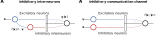
\includegraphics[trim=0cm 0cm 7.9cm 0cm,clip]{media/chapters/03_nlif/03_02/inhibitory_interneurons_overview.pdf}\hspace{0.4204cm}%
	\includegraphics[trim=0cm 0cm 7.9cm 0cm,clip]{media/chapters/03_nlif/03_02/inhibitory_interneurons.pdf}%
	{\phantomsubcaption\label{fig:inhibitory_interneurons_a}}%
	{\phantomsubcaption\label{fig:inhibitory_interneurons_b}}%
	\caption[Inhibitory interneurons]{Inhibitory interneurons.
	\textbf{(A)} To establish interneuron populations, we compute the identity function $f(x) = x$ in the purely excitatory projection onto the interneurons.
	The desired $\phi(\vec x)$ is then decoded from a virtual population encompassing both the inhibitory interneurons, and the excitatory pre-neurons.
	\textbf{(B)} Using this scheme, we can compute linear and nonlinear functions $\phi(x)$.
	Data for $100$ neurons per population with maximum firing rates between $50$ and $100\,\mathrm{Hz}$; weight matrices are determined by solving \cref{eqn:decode_nonneg} with $\sigma = 10$.
	The dotted line is the target $\phi(x)$, black line is the median decoded value over 1000 trials, shaded grey areas correspond to the 10th and 90th percentiles.
	Errors $E$ are the mean \NRMSE with standard deviation.
	}
	\label{fig:inhibitory_interneurons}
\end{figure}

\subsubsection{Inhibitory interneuons}
Connectivity patterns in biology do not suggest an arbitrary split of neural ensembles into excitatory and inhibitory neurons.
Instead, as we explained in \Cref{sec:nef_limitations}, excitatory signals are often mediated through interneurons that provide local inhibition \citep[e.g.,][Chapter~2]{kandel2012principles}.
\citet{parisien2008solving} suggest a way to 
construct \NEF networks with such inhibitory interneurons.

The techniques we discussed above can similarly be used to construct networks with inhibitory interneurons, albeit in a much simpler manner.
Recall that we can compute the identity function over purely excitatory connections (cf.~\Cref{fig:nonnegative_experiments}).
We can hence represent $\vec x$ in the interneurons using excitatory connection weights (cf.~\Cref{fig:inhibitory_interneurons_a}).
With this connection in place, the pre- and interneurons can be thought of as forming a \enquote{virtual pre-population} representing the same quantity $\vec x$.
Using \cref{eqn:decode_nonneg} we can solve for excitatory weights $\vec w_i^+$ originating from the pre-population, and inhibitory weights $\vec w_i^-$ originating from the interneurons, that project onto the post-population while approximating a function $\phi(\vec x)$.

Although we decode from multiple pre-populations, we do not need to resort to an optimisation problem such as \cref{eqn:decode_current_additive}, where we decoded additive functions from multiple pre-populations.
This is possible because both pre-populations represent the same value.
Hence, we do not require a double integral, and we can compute nonlinear functions over $\vec x$.

As depicted in \Cref{fig:inhibitory_interneurons_b}, we can use this technique to approximate linear and nonlinear functions $\phi(\vec x)$; errors mostly stem from the pre- to interneuron connection.
Crucially, in contrast to the \enquote{Parisien transform}, we did not take any special precautions regarding the interneuron tuning curve distributions.
All populations use the \enquote{standard} tuning with uniform $x$-intercepts.
This is possible because we solve for weights directly in current space.

\begin{figure}
	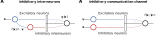
\includegraphics[trim=7.9cm 0cm 0cm 0cm,clip]{media/chapters/03_nlif/03_02/inhibitory_interneurons_overview.pdf}%
	\includegraphics[trim=7.9cm 0cm 0cm 0cm,clip]{media/chapters/03_nlif/03_02/inhibitory_interneurons.pdf}%
	{\phantomsubcaption\label{fig:inhibitory_comm_a}}%
	{\phantomsubcaption\label{fig:inhibitory_comm_b}}%
	\caption[Inhibitory communication channels]{Inhibitory communication channels.
	\textbf{(A)}~Inhibitory neurons can be used to form a communication channel, as long as there is some excitatory population that can provide a bias.
	\textbf{(B)}~Experiment demonstrating the use of this network setup as a communication channel.
	While the inhibitory connection is a good communication channel, nonlinear functions can only be computed with larger errors.
	All points are sampled from $(x, \nu) \in [-1, 1]^2$; the $\nu$-dimension is not depicted.
	See \Cref{fig:inhibitory_interneurons_b} for the network parameters and description of the depicted quantities.
	}
	\label{fig:inhibitory_comm}
\end{figure}

\subsubsection{Inhibitory communication channels}
Curiously, using the same techniques, we can also construct purely inhibitory communication channels---at least under the assumption that there is some separate excitatory pre-population that can be used as a bias source.
The lack of such an excitatory population is exactly what prevented us from computing functions across inhibitory connections in \Cref{fig:nonnegative_experiments}.

Given an inhibitory population representing $\vec x$, and another population representing some unrelated $\vec \nu$ (cf.~\Cref{fig:inhibitory_comm_a}).
Similar to \cref{eqn:decode_current_additive}, we minimise (without regularisation)
\begin{align}
	\min_{\vec w_i^+, \vec w_i^-}
	\frac{1}{\vol(\Xrepr)^2} \! \iint_{\Xrepr}
	\left(
		J_i\bigl(\langle \vec e_i, \phi(\vec x) \rangle\bigr)
		- \langle \vec w^-_i, -\vec a^-(\vec x) \rangle
		- \langle \vec w^+_i, \vec a^+(\vec \nu) \rangle
	\right)^2 \, d\vec x \, d\vec \nu %+ \sigma^2 \|\vec w_{i}^+\|_2^2 + \sigma^2 \|\vec w_{i}^-\|_2^2 \,,
	\label{eqn:inhibitory_communication_channel}
\end{align}
subject to $\vec w_{i}^+$, $\vec w_{i}^- > 0$.
Crucially, we ignore $\vec \nu$ in our target function; we solely use the pre-population to provide background activity but ignore its represented value.

Results of an experiment exploring this technique are depicted in \Cref{fig:inhibitory_comm_b}.
While computing the identity function---i.e., constructing a pure communication channel---works well, nonlinear functions can only be decoded with a considerable error, just as with purely excitatory channels (cf.~\Cref{fig:nonnegative_experiments}).
This is due to the standard \NEF pre-population tuning curves not providing a good basis for nonnegative decoding of many nonmonotonic functions.
In principle, it should be possible to have pre-population tuning such that any nonnegative target current function can be nonnegatively decoded with an arbitrarily small error.
An example would be the Gaussian tuning curves similar to those depicted in \Cref{fig:bias_decoding_impact_c}.

Inhibitory networks similar to what we discussed here are explored in some more detail by \citet{tripp2016function}.
However, as with the Parisien transform, this prior work relies on specific tuning of the inhibitory neurons, as well as intrinsic biases.

\subsection{Subthreshold Relaxation}
\label{sec:nef_subthreshold}

\begin{figure}
	\includegraphics{media/chapters/03_nlif/03_02/subthreshold_illustration.pdf}%
	{\phantomsubcaption\label{fig:subthreshold_illustration_a}}%
	{\phantomsubcaption\label{fig:subthreshold_illustration_b}}%
	{\phantomsubcaption\label{fig:subthreshold_illustration_c}}%
	\caption[Illustration of the goal of subthreshold relaxation]{Illustration of the goal of subthreshold relaxation.
	\textbf{(A)} Most neurons act as rectifiers. Input currents below $J_\mathrm{th}$ (grey) are mapped onto zero.
	\textbf{(B)} Five randomly generated tuning curves with uniform $x$-intercepts and maximum firing rates between $50$ and $100$ spikes per second.
	\textbf{(C)} Using affine current-translation functions $J_i(\xi)$, these tuning curves are generated by comparably large negative currents. However, the magnitude of the currents below $J_\mathrm{th}$ (grey) has no effect on the output rate; in fact any current below $J_\mathrm{th}$ has the same effect on the firing rate of the neuron.
	}
\end{figure}

Most biological model neurons act as rectifiers.
That is, input currents below a certain, usually positive, threshold $J_\mathrm{th}$ do not result in any output activity.
In the case of our simplified \LIF neuron model (cf.~\Cref{sec:simplified_neuron_models}), the threshold current $J_\mathrm{th}$ is \SI{1}{\nano\ampere} (\Cref{fig:subthreshold_illustration_a}).
We did not take this into account in our above current-space optimisation schemes.

To the contrary, our current-based loss functions in \cref{eqn:decode_current,eqn:decode_nonneg} aim at \emph{precisely} evoking certain post-synaptic currents $J_\mathrm{tar}$.
Notably, the negative currents required by the affine current translation function $J_i(\xi)$ can be larger in magnitude than the positive currents (\Cref{fig:subthreshold_illustration_b,fig:subthreshold_illustration_c}).
This has not been an issue in \NEF networks with intrinsic current-translation, as $J_i(\xi)$ takes care of appropriately scaling and offsetting the input currents.

However, in the context of our current-space optimisation schemes, a regularised least-squares optimisation problem can \enquote{prioritise} solving for exact (but irrelevant) subthreshold currents over solving for the (relevant) superthreshold currents.
This can lead to an increase in the superthreshold current-decoding error, and thus also increase the representation error in the post-population.
Additionally, as we will see below, dendritic nonlinearities impose asymptotic maximum and minimum post-synaptic currents.
Trying to solve for large negative currents may thus result in large connection weights.

One way to work around this issue is to clamp target currents $J_\mathrm{tar}$ that are substantially below the threshold to some constant.
For example, in the case of our simplified \LIF neuron, we could clamp all negative target currents to a current of zero.
This way, the solver does not have to generate the afforementioned large negative subthreshold currents.
Still, this \enquote{clamping} approach requires the weight solver to \emph{precisely} solve for the desired target current although \emph{any} subthreshold current would do.

Conceptually, it would be better to \enquote{relax} the requirement to solve for $J_\mathrm{tar}$ as precisely as possible for subthreshold currents.
Instead, we could merely demand that subthreshold target currents are decoded as subthreshold currents, regardless of the magnitude.
If this constraint is violated, i.e., if the target current $J_\mathrm{tar}$ is below the threshold and the decoded current $J_\mathrm{dec}$ is above the threshold $J_\mathrm{th}$, we measure the distance to the threshold, and not the distance to $J_\mathrm{tar}$ as an error.
We formalise this as a superthreshold error function $\mathcal{E}$,
\begin{align}
\mathcal{E}(J_\mathrm{tar}, \, J_\mathrm{dec}) = \begin{cases}
0 & \text{if } J_\mathrm{tar} < J_\mathrm{th} \text{ and } J_\mathrm{dec} < J_\mathrm{th} \,,\\
J_\mathrm{dec} - J_\mathrm{th} & \text{if } J_\mathrm{tar} < J_\mathrm{th} \text{ and } J_\mathrm{dec} > J_\mathrm{th} \,,\\
J_\mathrm{dec} - J_\mathrm{tar} & \text{if } J_\mathrm{tar} \geq J_\mathrm{th} \,,\\
\end{cases}
\label{eqn:subthreshold_error}
\end{align}
and define a new current-space optimisation problem akin to \cref{eqn:decode_nonneg}
\begin{align}
	\min_{\vec w_i^+, \vec w_i^-} 
	\frac{1}{\vol(\Xrepr)}
	\int_{\Xrepr} \mathcal{E}\left( 
		J_i(\langle \vec e_i, \phi(\vec x)\rangle),
		\langle \vec w_i^+, \vec a^+(\vec x) \rangle +
		\langle \vec w_i^-, -\vec a^-(\vec x) \rangle
	\right)^2 \, \D \vec x
	+ \sigma^2 \| \vec w^+_i \|_\mathrm{2}^2
	+ \sigma^2 \| \vec w^-_i \|_\mathrm{2}^2\,.
\label{eqn:decode_current_subthreshold}
\end{align}

\subsubsection{Subthreshold relaxation as a quadratic program}
It is not immediately clear how to solve this optimisation problem.
While, it is always possible to resort to gradient descent, \cref{eqn:decode_current_subthreshold} can be solved more efficiently by rewriting the loss function in terms of a convex \qprog (\QP).
\QPpl are a generalisation of least-squares and defined as follows:
\begin{definition}[Quadratic Program]
\label{def:qp}
A \emph{quadratic program} (\QP) is an optimisation problem of the form \citep[adapted in slightly simplified form from][Section~4.4]{boyd2004convex}
\begin{align*}
	\text{minimize} &\quad
		\vec \omega^T \mat P \vec \omega + \mat q^T \vec \omega \\
	\text{subject to} &\quad
		\mat G \vec \omega \leq \vec h \,,
\end{align*}
where $\vec \omega \in \mathbb{R}^{n}$, $\mat P \in \mathbb{R}^{n \times n}$, $\vec q \in \mathbb{R}^{n}$, $\mat G \in \mathbb{R}^{\ell \times n}$, $\vec h \in \mathbb{R}^{\ell}$.
Here, $n$ is the number of variables and $\ell$ is the number of inequality constraints.
If $\vec \omega^T \mat P \vec \omega$ is a convex function (i.e., $\mat P$ is positive definite) and the constraints $\mat G \vec \omega \leq \vec h$ form a convex polytope, then the QP is \emph{convex}.
\end{definition}

Convex \qprogpl can be solved in polynomial time \citep{kozlov1980polynomial}.
There are free and open-source software libraries, such as \enquote{cvxopt} \citep{vandenberghe2010cvxopt} and \enquote{OSQP}  \citep{stellato2020osqp} that solve such problems efficiently.
In our experiments we mostly rely on OSQP.%
\footnote{Some experiments were conducted before OSQP was published; we used cvxopt in those experiments. We did not observe any discernible difference in the solutions produced by the two libraries, but as a C library using more modern algorithms, OSQP is substantially faster than the older Python library cvxopt.}

To transform a discretised version of \cref{eqn:decode_current_subthreshold} into a \qprog we split the sample points $\vec x_k$ according to whether they evoke super- or subthreshold currents.
Specifically, we arrange the pre-activities $\mat A$ and target currents $\mat J$ as follows:
\begin{align*}
	\mat{A}_\mathrm{sup} = (
		  \mat{A}^+_\mathrm{sup}, 
		- \mat{A}^-_\mathrm{sup})
		\in
		\mathbb{R}^{N_\mathrm{sup} \times (n^+ + n^-)} \,,
	&&
	\mat{J}_\mathrm{sup} \in \mathbb{R}^{N_\mathrm{sup}} \,,
	&&
	\mat{A}_\mathrm{sub} = (
		  \mat{A}^+_\mathrm{sub}, 
		- \mat{A}^-_\mathrm{sub})
		\in
		\mathbb{R}^{N_\mathrm{sub} \times (n^+ + n^-)} \,.
\end{align*}
Here, $N_\mathrm{sup}$, $N_\mathrm{sub}$ with $N = N_\mathrm{sup} + N_\mathrm{sup}$
are the number of samples with a super- and subthreshold target currents, and, as before, $n^+$ and $n^-$ correspond to the number of excitatory and inhibitory pre-neurons.
Using these matrices, \cref{eqn:decode_current_subthreshold} can be expressed as a \QP by letting
\begingroup
\setlength\fboxsep{2pt}
\newcommand{\cA}{LightSkyBlue}
\newcommand{\cB}{Plum}
\newcommand{\cC}{Salmon}
\newcommand{\cD}{Khaki}
%\newcommand{\hlA}[1]{\colorbox{\cA}{\ensuremath{#1}}}
%\newcommand{\hlB}[1]{\colorbox{\cB}{\ensuremath{#1}}}
%\newcommand{\hlC}[1]{\colorbox{\cC}{\ensuremath{#1}}}
%\newcommand{\hlD}[1]{\colorbox{\cD}{\ensuremath{#1}}}
\newcommand{\hlA}[1]{{\ensuremath{#1}}}
\newcommand{\hlB}[1]{{\ensuremath{#1}}}
\newcommand{\hlC}[1]{{\ensuremath{#1}}}
\newcommand{\hlD}[1]{{\ensuremath{#1}}}
\begin{align}
	\mat P &= \begin{pmatrix}
		  \hlA{(\mat A_\mathrm{sup})^T \mat A_\mathrm{sup} + N \sigma^2 \mat I)}
		& 0 \\
		  0
		& \hlB{\mat I}
	\end{pmatrix} ,
	&
	\!\!\! \vec q &= \begin{pmatrix}
		\hlA{(\mat A_\mathrm{sup})^T \vec J_\mathrm{sup}} \\
	0
	\end{pmatrix} ,
	&
	\!\!\! \mat G &= \begin{pmatrix}
		\hlC{\mat A_\mathrm{sub}} & \hlB{\mat I} \\
		\hlD{-\mat I} & 0
	\end{pmatrix} ,
	&
	\!\!\! \vec h &= \begin{pmatrix}
		\hlC{\vec{J}_\mathrm{th}} \\
		\hlD{0}
	\end{pmatrix} .
	\label{eqn:decode_subthreshold_qp}
\end{align}
The number of variables is $n = n^+ + n^- + N_\mathrm{sub}$, and the number of inequality constraints is $\ell = N_\mathrm{sub} + n^+ + n^-$.
The parameter vector $\vec \omega \in \mathbb{R}^{n}$ can be split into the excitatory and inhibitory weights $\vec w_i^+ \in \mathbb{R}^{n^+}$, $\vec w_i^- \in \mathbb{R}^{n^-}$, as well as discardable slack variables $\vec s_i \in \mathbb{R}^{N_\mathrm{sub}}$.

The rationale behind \cref{eqn:decode_subthreshold_qp} is as follows.
The first line of $\mat P$ and $\vec q$
%(${\color{\cA}\blacksquare}$)
is the standard regularised least-squares problem obtained by expanding the superthreshold potion of \cref{eqn:decode_current_subthreshold} (cf.~\cite{boyd2004convex}, Section~4.4).
The first column and row of $\mat G$ and $\vec h$
%(${\color{\cC}\blacksquare}$)
add an inequality constraint that ensures that samples with subthreshold currents are decoded as subthreshold currents.
Violations of this constraint, i.e., case two of \cref{eqn:subthreshold_error}, are enabled by the slack variables $\vec s_i$ (second column of $\mat P$ and $\mat G$%
%; ${\color{\cB}\blacksquare}$
).
These slack variables correspond to the error $J_\mathrm{th} - J_\mathrm{tar}$, which is penalised accordingly in $\mat P$.
Finally, nonnegativity of the weights is ensured by the second row of $\mat G$ and $\vec h$%
% (${\color{\cD}\blacksquare}$)
. One can easily show that this \QP is convex.
\endgroup

\begin{figure}
	\includegraphics{media/chapters/03_nlif/03_02/subthreshold_comparison.pdf}%
	{\phantomsubcaption\label{fig:subthreshold_comparison_a}}%
	{\phantomsubcaption\label{fig:subthreshold_comparison_b}}%
	{\phantomsubcaption\label{fig:subthreshold_comparison_c}}%
	{\phantomsubcaption\label{fig:subthreshold_comparison_d}}%
	\caption[Current decoding with and without subthreshold relaxation]{Current decoding with and without subthreshold relaxation in a setting with low regularisation ($\sigma = 0.31$) and few pre-neurons ($n = 50$).
	Values above each plot are the \RMS of the superthreshold error ${\mathcal{E}}$ (eq.~\ref{eqn:subthreshold_error}).
	Subthreshold relaxation substantially reduces the decoding error.	
	}
	\label{fig:subthreshold_comparison}
\end{figure}

\subsubsection{Example: Individual post-neuron}
In \Cref{fig:subthreshold_comparison} we decode the post-synaptic currents for a single post neuron using \NNLS, \NNLS with clamped target currents, and subthreshold relaxation.
At least in this example, subthreshold relaxation substantially reduces the superthreshold decoding error.
In contrast, clipping the target currents has only a limited positive effect.
Notably, and particularly pronounced in the case of purely excitatory pre-neurons, the solution obtained with subthreshold relaxation is supported by more pre-neurons.
This is visible in \Cref{fig:subthreshold_comparison_c}, where subthreshold relaxation decodes a non-zero current for negative $\xi$, resulting in a smaller regularisation error (i.e., weight \RMS of $0.8 \times 10^{-3}$ vs. $2 \times{10}^{-3}$).

\begin{figure}[t]
	\includegraphics{media/chapters/03_nlif/03_02/subthreshold_experiment.pdf}%
	{\phantomsubcaption\label{fig:subthreshold_experiment_a}}%
	{\phantomsubcaption\label{fig:subthreshold_experiment_b}}%
	{\phantomsubcaption\label{fig:subthreshold_experiment_c}}%
	\caption[Reduction in decoding error achieved with subthreshold relaxation]{Reduction in decoding error achieved with subthreshold relaxation compared to standard \NNLS and clipping the target current.
	\textbf{(A)} Reduction in the decoded post-synaptic currents error relative to \NNLS for different thresholds in the error measure $\mathcal{E}$.
	Each box plot over three functions, $100$ random networks, $11$ noise magnitudes, and $9$ random samplings of the noise ($N = 29\,700$); whiskers are the extrema, boxes the quartiles, orange line is the median, green dashed line the mean.
	\textbf{(B)}
	Same as \emph{(A)}, but for the post-population decoding error.
	\textbf{(C)} Same data as above, but over different pre-population noise magnitudes and for different functions $\phi(x)$ computed in the pre to post connection.
	Coloured lines show the median error (see \emph{(A, B)} for a legend); shaded areas are the 25\% and 75\% quartiles.
	}
	\label{fig:subthreshold_experiment}
\end{figure}

\subsubsection{Systematic experiment}
One issue with subthreshold relaxation is that not solving for strongly negative currents can result in a narrower separation boundary between the threshold and the decoded current.
Hence, noise on the pre-activities is more likely to result in positive post-activity.
However, this may be compensated for by the smaller regularisation error, and hence higher robustness to noise as observed in the previous example.

\Cref{fig:subthreshold_experiment} depicts the results of a more systematic experiment.
We compute three polynomials in the connection between one hundred pre and post \LIF rate neurons ($1\!\!:\!\!1$ excitatory to inhibitory ratio) with varying degree of Gaussian noise added to the pre-activities.
We select the regularisation factor $\sigma$ to minimise the error for the given amount of noise on a separate training set.
We furthermore vary the threshold $J_\mathrm{th}$ assumed in \cref{eqn:subthreshold_error}, to investigate the effect of moving $J_\mathrm{th}$ away from the true threshold.

As visible in \Cref{fig:subthreshold_experiment_a}, subthreshold relaxation reduces the current decoding error by about 50\% (median), largely independent of the assumed $J_\mathrm{th}$.
Clamping the currents leads to a reduction in error with a median of about 35\%, but, overall, the reduction in error is less consistent.
Improvements to the representation accuracy (\Cref{fig:subthreshold_experiment_b}) are less drastic, with the largest improvement for $J_\mathrm{th} = \SI{0.75}{\nano\ampere}$ with a median reduction in error of about 13\%.
This confirms our suspicion that setting $J_\mathrm{th}$ to the true threshold can be slightly detrimental.

This is further confirmed by the experiment in \Cref{fig:subthreshold_experiment_c} where we plot the post-population representation error over different pre-activity noise magnitudes.
For small amounts of noise subthreshold relaxation with $J_\mathrm{th} = \SI{1}{\nano\ampere}$ can lead to large improvements in the representation error; however, for larger noise magnitudes the overall benefit of subthreshold relaxation is smaller, with slightly reduced $J_\mathrm{th}$ performing the best.
%We provide additional results from this experiment in Appendix C.2.

Keep in mind that \LIF \emph{rate} neurons are a worst-case scenario with respect to sensitivity to pre-activity noise injected near the threshold.
\LIF rate neurons possess a very steep activity onset, where small changes in current lead to large fluctuations in activity.
This tends to be less of an issue with transient noise in spiking neural networks, which results in a smoother response curve (see our discussion below, as well as \cite{hunsberger2015spiking}).
We can thus expect that, in practice, the impact of subthreshold relaxation is somewhere between the values obtained for the current decoding and representation error.

\subsection{Extension Toward Dendritic Nonlinearities}
\label{sec:nef_nonlinear}

Up to this point we assumed current-based synapses.
As previously discussed in \Cref{sec:dendritic_computation_theory}, the defining property of current-based synapses is that the somatic current $J$ is linear in the synaptic weights $\vec w$ and the pre-synaptic activities $\vec a$, that is $a_i = G[J] = G[\langle \vec w, \vec a \rangle]$.
In contrast, we described neurons with nonlinear synapses as follows
\begin{align}
	a_i &=
	\mathscr{G} \bigl[
		g_i^1, \ldots, g_i^k
	\bigr] =
	\mathscr{G} \bigl[
		\langle \vec w_{i}^1, \vec a_1 \rangle,
		\ldots ,
		\langle \vec w_{i}^k, \vec a_k \rangle
	\bigr] \,.
	\label{eqn:def_response_curve_g}
\end{align}
Here, $k$ is the number of input channels, and the vector $\vec g_i = (g^1_i$, $\ldots$, $g^k_i)$ describes some abstract \enquote{channel state}.
Again, we assume that, on average, each channel state $g^j_i$ is linear in the weights and the activities $\vec a_j$ of the neurons connecting to the $j$th channel.
However, we do not make any assumption regarding the effect of $g^j_i$ on the somatic current $J$; more fundamentally, we do not assume that there exists an easily identifiable somatic current at all.

The lack of an identifiable somatic current makes it more challenging to integrate such neurons into the \NEF.
The optimisation problems we discussed in this section relied on the current translation function $J_i(\xi)$ to enforce the normative tuning constraint $a_i(\vec x)$.
Of course, as mentioned above, we could resort to gradient descent to optimise \cref{eqn:dendritic_computation_optimisation}.
However, our current-based optimisation schemes work well in that they allow us to quickly solve for globally optimal weights.
As we will see, it is still possible to perform global current-space optimisation for some multi-channel neurons.
Additionally, we can use the same ideas to iteratively solve for locally optimal weights in more complex multi-compartment neurons.

\begin{figure}
	\centering
	\includegraphics{media/chapters/03_nlif/03_02/two_compartment_response_curve.pdf}
	\caption[Neural response curve decomposition]{Neural response curve decomposition. \textbf{(A)} Illustration of the multivariate neuron response curve $\mathscr{G}(g_\mathrm{E}, g_\mathrm{I})$ for a two-compartment \LIF neuron with excitatory and inhibitory conductance-based channels. \textbf{(B, C)} The chosen somatic nonlinearity $G$ and its inverse $G^{-1}$. \textbf{(D)} corresponding input-dependent nonlinearity $H$. The neuron does not fire in the hatched regions, that is, $G^{-1}$ is ill-defined.} 
	\label{fig:two_compartment_response_curve}
\end{figure}

To this end, the crucial idea is to mathematically reintroduce a \enquote{virtual} somatic current $J$ by decomposing $\mathscr{G}$ into the standard somatic nonlineartiy $G$ and a dendritic nonlinearity $H$.

\begin{definition}[Dendritic Nonlinearity]
\label{def:dendritic_nonlinearity}
Given a neural response curve $G$, the \emph{dendritic nonlinearity} $H(\vec g_i)$ of a multi-channel neuron with response curve $\mathscr{G}$ maps the input channel state $\vec g_i = (g^1_i, \ldots, g^k_i)$ onto an \emph{average}, time-independent somatic current $J$ such that
\begin{align}
		H\big(g^1_i, \ldots, g^k_i\big) = J
	\Leftrightarrow
		G\big[J\big] = \mathscr{G}\big[g^1_i, \ldots, g^k_i\big] 
	\Leftrightarrow
		\mathscr{G}\big[g^1_i, \ldots, g^k_i\big] = G\big[H(g^1_i, \ldots, g^k_i)\big] \,.
	\label{eqn:def_h}
\end{align}
\end{definition}
Optimally, $G$ is chosen such that $H$ is as simple as possible.
For example, if the neuron model is an extension to a \LIF neuron, $G$ can be the standard \LIF response curve.
In this case, $H$ translates the input into an \enquote{\LIF-equivalent current}.
In the trivial case of the above current-based \LIF neurons with excitatory and inhibitory inputs, we would obtain $H(J_\mathrm{E}, J_\mathrm{I}) = J_\mathrm{E} - J_\mathrm{I}$.

We use the dendritic nonlinearity $H$ to define a new current-space loss function
\begin{align}
	E = \frac{1}{\vol(\Xrepr)} \int_{\Xrepr}
		\mathcal{E} \bigl(
			J_i(\langle \vec e_i, f(\vec x_k) \rangle),
			H(\langle \vec w^1_i, \vec a^k \rangle, \ldots, \langle \vec w^k_i, \vec a^k \rangle)
		\bigr)^2 \,\mathrm{dx} + \sigma^2 \sum_{j = 1}^\ell \| \vec w^j_i \|_2^2\,,
\label{eqn:decode_nonlinear_synapses}
\end{align}
where $\mathcal{E}$ is the superthreshold error defined in \cref{eqn:subthreshold_error}, $\vec a^j$ are the pre-activities, and connection weights $\vec w_i$ may be---depending on the input channel type---nonnegative.

We next show that it is possible to derive $H$, or at least a suitable surrogate model, in closed form for multi-compartment \LIF neurons with conductance-based synapses.
If $H$ cannot be derived in closed form, we can sample $\mathscr{G}$ over varying synaptic states and, as depicted in \Cref{fig:two_compartment_response_curve}, compute $H$ indirectly by applying an inverse mapping $G^{-1}$ to the recorded data.
